% LaTeX source for PyMS User Guide

\documentclass[twoside,a4paper]{book}

\usepackage{epsfig}
\usepackage{graphicx}
\usepackage{makeidx}
\usepackage{tlk2e/tlk2e}
\usepackage{url}

\setlength{\topmargin}{0.0cm}
\setlength{\evensidemargin}{0.0cm}
\setlength{\oddsidemargin}{0.0cm}
\setlength{\textwidth}{16.0cm}
\setlength{\textheight}{23.0cm}
%\setlength{\footskip}{0.0cm}

\parskip 0.2cm
\parindent 0cm
\makeindex

\begin{document}

\frontmatter

\title{\includegraphics{logo/PyMS.eps}
\Large{PyMS User Guide}}
\author{Andrew Isaac and Vladimir Liki\'{c}\\
with contributions from:\\
\medskip}

\medskip

\version{PyMS version 1.0}

\abstract{A Python toolkit for processing of chromatography--mass spectrometry
data}

\maketitle
\tableofcontents

\input epsf

\newpage

\setcounter{chapter}{1}
\setcounter{section}{0}
\pagenumbering{arabic}
% chapter01.tex

 %%%%%%%%%%%%%%%%%%%%%%%%%%%%%%%%%%%%%%%%%%%%%%%%%%%%%%%%%%%%%%%%%%%%%%%%%%%%%
 %                                                                           %
 %    PyMS2 documentation                                                     %
 %    Copyright (C) 2005-8 Vladimir Likic                                    %
 %                                                                           %
 %    The files in this directory provided under the Creative Commons        %
 %    Attribution-NonCommercial-NoDerivs 2.1 Australia license               %
 %    http://creativecommons.org/licenses/by-nc-nd/2.1/au/                   %
 %    See the file license.txt                                               %
 %                                                                           %
 %%%%%%%%%%%%%%%%%%%%%%%%%%%%%%%%%%%%%%%%%%%%%%%%%%%%%%%%%%%%%%%%%%%%%%%%%%%%%

\chapter{Introduction}

\section{About PyMS2}

PyMS2 is a Python toolkit for processing of chromatography--mass spectrometry
data. The main idea behind PyMS2 is to provde a framework and a set of
components for rapid development and testing of methods for processing of
chromatography--mass spectrometry data. An important objective of PyMS2 is
to decouple processing methods form visualization and the concept of
interactive processing. This is useful for high-throughput processing tasks
and when there is a need to run calculations in the batch mode.

PyMS2 is modular and consists of several sub-packages written in Python
programming language \cite{python}. PyMS2 is released as open source,
under the GNU Public License version 2.

There are four parts of the pyms project:

\begin{itemize}
  \item pyms2 -- The PyMS2 code
  \item pyms2-docs -- The PyMS2 documentation
  \item pyms2-test -- Examples of PyMS2 use
\end{itemize}

Each part is a separate project on Google Code that can be downloaded
separately. The data used in PyMS2 documentation and examples is available
from the Bio21 Institute server:\\
{\tt http://bioinformatics.bio21.unimelb.edu.au/pyms-data/}\\
In addition, the current PyMS2 API documentation is available from here:\\
{\tt http://bioinformatics.bio21.unimelb.edu.au/pyms.api/index.html}

\section{PyMS2 installation}

There are several ways to install PyMS2 depending your computer configuration
and preferences. The recommended way install PyMS2 is to compile Python
from sources and install PyMS2 within the local Python installation. This
procedure is described below.

PyMS2 has been developed on Linux, and a detailed installation instructions
for Linux are given below. Installation on any Unix-like system should be
similar. We have not tested PyMS2 under Microsoft Windows.

\subsection{Downloading PyMS2 source code}

PyMS2 source code resides on Google Code servers, and can be accessed
from the following URL: http://code.google.com/p/pyms/. Under the
section "Source" one can find the instructions for downloading the
source code. The same page provides the link under "This project's
Subversion repository can be viewed in your web browser" which allows
one to browse the source code on the server without actually downloading
it.

Google Code maintains the source code with the program 'subversion'
(an open-source version control system). To download the source code
one needs to use the subversion client program called 'svn'. The 'svn'
client exists for all mainstream operating systems\footnote{For example,
on Linux CentOS 4 we have installed the RPM package
'subversion-1.3.2-1.rhel4.i386.rpm' to provide us with the subversion
client 'svn'.}, for more information see http://subversion.tigris.org/.
The book about subversion is freely available on-line at
http://svnbook.red-bean.com/. Subversion has extensive functionality.
However only the very basic functionality is needed to download PyMS2
source code.

If the computer is connected to the internet and the subversion client
is installed, the following command will download the latest PyMS2 source
code:

\begin{verbatim}
$ svn checkout http://pyms.googlecode.com/svn/trunk/ pyms
A    pyms/Peak
A    pyms/Peak/__init__.py
A    pyms/Peak/List
A    pyms/Peak/List/__init__.py
.....
Checked out revision 71.
\end{verbatim}

\subsection{PyMS2 installation}

PyMS2 installation consists of placing the PyMS2 code directory (pyms/) in
place visible to Python interpreter.  This can be in the standard place
for 3rd party software (the directory site-packages/). If PyMS2 code is
placed in a non-standard place the Python interpreter needs to be made
aware of it before before it is possible to import PyMS2 modules (see the
Python sys.path.append() command).

We recommend compiling your own Python installation for PyMS2.

In addtion to the PyMS2 core source code, a number of external packages
is used to provide additional functionality. These are explained below.

\subsection{\label{subsec:numpy}Package 'NumPy'}

The package NumPy is provides numerical capabilities to Python. This
package is used throughout PyMS2 (and also required for some external
packages used in PyMS2), to its installation is mandatory. 

The NumPy web site {\tt http://numpy.scipy.org/} provides the installation
instructions and the link to the source code.

\subsection{\label{subsec:pycdf}Package 'pycdf' (required for reading
ANDI-MS files)}

The pycdf (a python interface to Unidata netCDF library) source and
installation instructions can be downloaded from
{\tt http://pysclint.sourceforge.net/pycdf/}. Follow the installation
instructions to install pycdf. 

\subsection{\label{subsec:pycluster}Package 'Pycluster' (required for peak
alignment by dynamic programming)}

The peak alignment by dynamic programming is located in the subpackage
pyms.Peak.List.DPA. This subpackage used the Python package 'Pycluster'
as the clustering engine. Pycluster with its installation instructions
can be found here:
{\tt http://bonsai.ims.u-tokyo.ac.jp/~mdehoon/software/cluster/index.html}.

\subsection{\label{subsec:scipy-ndmage}Package 'scipy.ndimage' (required
for TopHat baseline correction)}

If the full SciPy package is installed the 'ndimage' will be available. However
the SciPy contains large amount of functionality, and its intallation is
somewhat involved. In some situations in may be preferable to install only
the subpackage 'ndimage'. The UrbanSim web site \cite{urbansim} provides
instructions how to install a local copy of 'ndimage'. These instructions
and the link to the file 'ndimage.zip' are here:\\
{\tt http://www.urbansim.org/opus/releases/opus-4-1-1/docs/installation/scipy.html}

\section{Current PyMS2 development environment}

PyMS2 is currently being developed with the following packages:

\begin{verbatim}
Python-2.5.2
numpy-1.1.1
netcdf-4.0
pycdf-0.6-3b
Pycluster-1.41
\end{verbatim}

A quick installation guide for packages required by PyMS2 is given below.

\begin{enumerate}

\item Python installation:

\begin{verbatim}
$ tar xvfz Python-2.5.2.tgz
$ cd Python-2.5.2
$ ./configure
$ make
$ make install
\end{verbatim}

\noindent
This installs python in /usr/local/lib/python2.5.  Make sure that python called
from the command line is the one just compiled and installed.

\item NumPy installation:

\begin{verbatim}
$ tar xvfz numpy-1.1.1.tar.gz
$ cd numpy-1.1.1
$ python setup.py install
\end{verbatim}

\item pycdf installation

Pycdf has two dependencies: the Unidata netcdf library and NumPy. The NumPy
installation is described above. To install pycdf, the netcdf library must
be downloaded ({\tt http://www.unidata.ucar.edu/software/netcdf/index.html}),
compiled and istalled first:

\begin{verbatim}
$ tar xvfz netcdf.tar.gz
$ cd netcdf-4.0
$ ./configure
$ make
$ make install
\end{verbatim}

The last step will create several binary 'libnetcdf*' files in /usr/local/lib.
pycdf can be installed as follows:

\begin{verbatim}
$ tar xvfz pycdf-0.6-3b
$ cd pycdf-0.6-3b
$ python setup.py install
\end{verbatim}

\item Pycluster installation

\begin{verbatim}
$ tar xvfz Pycluster-1.42.tar.gz
$ cd Pycluster-1.42
$ python setup.py install
\end{verbatim}

\item ndimage installation:

\begin{verbatim}
$ unzip ndimage.zip
$ cd ndimage
$ python setup.py install --prefix=/usr/local
\end{verbatim}

\noindent
Since ndimage was installed outside the scipy package, this requires some manual
correction:

\begin{verbatim}
$ cd /usr/local/lib/python2.5/site-packages
$ mkdir scipy
$ touch scipy/__init__.py
$ mv ndimage scipy
\end{verbatim}

\end{enumerate}

\section{Troubleshootings}

The PyMS2 is essentially a python library (a 'package' in python parlance, which
consists of several 'sub-packages'), which for some functionality depends on
other python libraries, such as NumPy, pycdf, and Pycluster. The most likely
problem with PyMS2 installation is a problem with installing one of the PyMS2
dependencies.

\subsection{Pycdf import error}

On Red Hat Linux 5 the SELinux is enabled by default, and this causes the
following error while trying to import properly installed pycdf: 

\begin{verbatim}
$ python
Python 2.5.2 (r252:60911, Nov  5 2008, 16:25:39)
[GCC 4.1.1 20070105 (Red Hat 4.1.1-52)] on linux2
Type "help", "copyright", "credits" or "license" for more information.
>>> import pycdf
Traceback (most recent call last):
  File "<stdin>", line 1, in <module>
  File "/usr/local/lib/python2.5/site-packages/pycdf/__init__.py", line 22, in <module>
    from pycdf import *
  File "/usr/local/lib/python2.5/site-packages/pycdf/pycdf.py", line 1096, in <module>
    import pycdfext as _C
  File "/usr/local/lib/python2.5/site-packages/pycdf/pycdfext.py", line 5, in <module>
    import _pycdfext
ImportError: /usr/local/lib/python2.5/site-packages/pycdf/_pycdfext.so:
    cannot restore segment prot after reloc: Permission denied
\end{verbatim}

This problem is removed simply by disabling SELinux (login as 'root', open the menu
Administration $\rightarrow$ Security Level and Firewall, tab SELinux, change settings
from 'Enforcing' to 'Disabled').

This problem is likely to occur on Red Hat Linux derivative distributions such as CentOS.



\setcounter{chapter}{2}
\setcounter{section}{0}
\pagenumbering{arabic}
% chapter02.tex

 %%%%%%%%%%%%%%%%%%%%%%%%%%%%%%%%%%%%%%%%%%%%%%%%%%%%%%%%%%%%%%%%%%%%%%%%%%%%%
 %                                                                           %
 %    PyMS documentation                                                     %
 %    Copyright (C) 2005-8 Vladimir Likic                                    %
 %                                                                           %
 %    The files in this directory provided under the Creative Commons        %
 %    Attribution-NonCommercial-NoDerivs 2.1 Australia license               %
 %    http://creativecommons.org/licenses/by-nc-nd/2.1/au/                   %
 %    See the file license.txt                                               %
 %                                                                           %
 %%%%%%%%%%%%%%%%%%%%%%%%%%%%%%%%%%%%%%%%%%%%%%%%%%%%%%%%%%%%%%%%%%%%%%%%%%%%%

\chapter{Using PyMS}

\section{Introduction}

The setup used for the examples below is as follows. The projects 'pyms',
'pyms-test', 'pyms-docs', and 'pyms-data' were downloaded in the directory
{\tt /home/current/proj/PyMS}. In the project 'pyms-test' there is a directory
corresponding to each example coded with the example number (ie.
{\tt pyms-test/01/} corresponds to Example 1). In each example directory
there is a script named 'proc.py' which contains the commands given in
the example. Provided that the paths to 'pyms' and 'pyms-data' are set
properly, these scripts could be run by simply:

\$ python proc.py

Before running each example the Python interpreter was made aware of the
PyMS location with the following commands:

\begin{verbatim}
import sys
sys.path.append("/home/current/proj/PyMS/")
\end{verbatim}

For brevity these commands will not be shown in the examples below, but
they are included in 'pyms-test' example scripts.  The above path need
to be adjusted to match your own location of pyms.

All data files (raw data files, peak lists etc) used in the example below
can be found in 'pyms-data'.


\section{Example 1: Reading of GC-MS data and basic manipulations}

\subsection{Reading ChemStation GC-MS data into PyMS}

The PyMS package pyms.IO provides capabilities to read the raw GC-MS
data stored in the ANDI-MS format. The function IO.ANDI.ChemStation()
provides the interface to ANDI-MS data files saved from Agilent
ChemStation software.\footnote{ANDI-MS data format stands for Analytical
Data Interchange for Mass Spectrometry, and was developed for the
description of mass spectrometric data developed in 1994 by Analytical
Instrument Association. ANDI-MS is essentially a recommendation, and
it is up to individual vendors of mass spectrometry processing software
to implement "export to ANDI-MS" feature in their software.}

The file '0510\_217.CDF' is a GC-MS experiment exported from Agilent
ChemStation (located in 'pyms-data'). This file can be loaded in the
memory as follows:

\begin{verbatim}
>>> from pyms.IO.ANDI.Class import ChemStation
>>> andi_file = "/home/current/proj/PyMS/pyms-data/0510_217.CDF"
>>> andi_data = ChemStation(andi_file)
 -> Processing netCDF file '/home/current/proj/PyMS/pyms-data/0510_217.CDF'
    [ 2784 scans, masses from 50 to 550 ]
>>>
\end{verbatim}

\noindent
The above command creates the object 'andi\_data' which is an {\em instance}
of the class IO.ANDI.ChemStation.

\subsection{Exploring an ANDI-MS data object}

The object 'andi\_data' has several attributes and methods associated with it.

\begin{verbatim}
>>> print "ANDI-MS data filename:", andi_data.get_filename()
ANDI-MS data filename: /home/current/proj/PyMS/pyms-data/0510_217.CDF
\end{verbatim}

The method {\tt get\_tic()} return total ion chromatogram (TIC) of the data
as an IonChromatogram object:

\begin{verbatim}
tic = andi_data.get_tic()
\end{verbatim}

\noindent
An IonChromatogram object is a one dimensional vector containing
mass intensities as a function of retention time. This can can be either
m/z channel intensities (for example, ion chromatograms at m/z = 65),
or cumulative intensities over all measured m/z (TIC).

The method {\tt get\_ic\_at\_index(i)} returns i-th ion chromatogram, as
an IonChromatogram object. For example, to get the first ion chromatogram
from the data:

\begin{verbatim}
ic = andi_data.get_ic_at_index(1)
\end{verbatim}

The method {\tt get\_ic\_at\_mass(MZ)} returns the ion chromatogram for
m/z = MZ.  For example, to get the ion chromatogram that corresponds
to m/z = 73:

An ion chromatogram object has a method {\tt is\_tic()} which returns
True is the ion chromatogram is TIC, False otherwise:

\begin{verbatim}
>>> print "'tic' is a TIC:", tic.is_tic()
'tic' is a TIC: True
>>> print "'ic' is a TIC:",ic.is_tic()
'ic' is a TIC: False
\end{verbatim}

\subsection{Writing data to a file}

The method {\tt write()} of IonChromatogram object allows one to save
the ion chromatogram object to a file:

\begin{verbatim}
>>> tic.write("output/tic.dat")
>>> ic.write("output/ic.dat")
\end{verbatim}

The method {\tt get\_intensity\_matrix()} of ChemStation object returns
the entire matrix of intensities:

\begin{verbatim}
>>> im = andi_data.get_intensity_matrix()
>>> print "Dimensions of the intensity matrix are:",len(im),"x",len(im[0])
Dimensions of the intensity matrix are: 2784 x 501
\end{verbatim}

\noindent
This data matrix contains 2784 time points (MS scans), and each time point
corresponds to a mass spectrum of 501 m/z points.

The intensity matrix can be saved to a file with the function 'save\_data()':

\begin{verbatim}
save_data("output/im.dat", im)
\end{verbatim}

The entire data (ie. ChemStation object) can be saved as CSV with the method
{\tt export\_csv()}. For example,

\begin{verbatim}
>>> andi_data.export_csv("output/data")
\end{verbatim}

\noindent
will create 'data.im.csv, data.mz.csv, and data.rt.csv where these are the
intensity matrix, retention time vector, and m/z vector in the CSV format.


\subsection{Using Octave or Matlab to plot the data}

The ion chromatogram object saved with with the {\tt write{}} method is a
plain ASCII file which contains a pair of (retention time, intensity) per
line:

\begin{verbatim}
$ cat tic.dat
 305.666      745997
 306.009      726566
 306.352      717704
 306.695      684214
 307.038      701866
 307.381      893306
 307.724     1278099
 308.067     1290984
 308.410      925558
 308.752      644122
[..output deleted..]
\end{verbatim}

\noindent
The left column is the retention time in seconds, while the right column
is the corresponding intensity. This data can be conveniently loaded and
plotted in matlab or octave:

\begin{verbatim}
octave:1> load tic.dat
octave:2> plot(tic(:,1)/60, tic(:,2))
\end{verbatim}

The output is shown in Figure \ref{ticplot}. In the above command the
time was divided by 60 to convert the x-axis into minutes.

\begin{figure}[htp]
\begin{center}
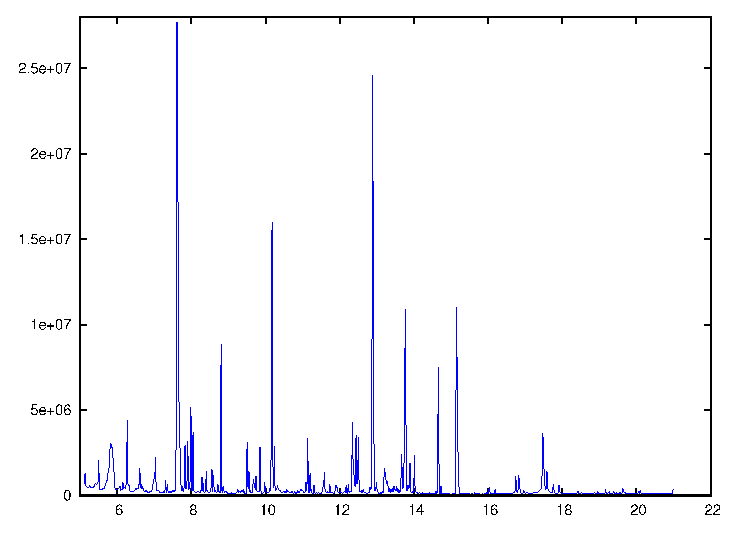
\includegraphics{graphics/tic.eps}
\caption{The octave plot of the file 'tic.dat'.}
\label{ticplot}
\end{center}
\end{figure}



\setcounter{chapter}{3}
\setcounter{section}{0}
\pagenumbering{arabic}
% chapter03.tex

 %%%%%%%%%%%%%%%%%%%%%%%%%%%%%%%%%%%%%%%%%%%%%%%%%%%%%%%%%%%%%%%%%%%%%%%%%%%%%
 %                                                                           %
 %    PyMS documentation                                                     %
 %    Copyright (C) 2005-8 Vladimir Likic                                    %
 %                                                                           %
 %    The files in this directory provided under the Creative Commons        %
 %    Attribution-NonCommercial-NoDerivs 2.1 Australia license               %
 %    http://creativecommons.org/licenses/by-nc-nd/2.1/au/                   %
 %    See the file license.txt                                               %
 %                                                                           %
 %%%%%%%%%%%%%%%%%%%%%%%%%%%%%%%%%%%%%%%%%%%%%%%%%%%%%%%%%%%%%%%%%%%%%%%%%%%%%

\chapter{Data pre-processing}

\section{Noise smoothing in ion chromatograms}

\noindent
[ {\em This example is in pyms-test/11} ]

Noise smoothing is usually the first step in raw data pre-processing. The
purpose of noise smoothing is to remove high-frequency noise from data, and
thereby increase the contribution of the signal relative to the contribution
of the noise.

One simple approach to noise smoothing is moving average window smoothing.
In this approach a window of fixed size $2N+1$ points is moved across the ion
chromatogram, and the value at each point is replaced with the mean intensity
over the window size. The pyms-test/11/ illustrates this. The script proc.py
is given below:

\begin{verbatim}
01  """proc.py
02  """
03  
04  import sys
05  sys.path.append("/home/current/proj/PyMS/")
06  
07  from pyms.IO.ANDI.Class import ChemStation
08  from pyms.Noise.Window import window_smooth
09  
10  andi_file = "/home/current/proj/PyMS/pyms-data/a0806_140.CDF"
11  andi_data = ChemStation(andi_file)
12  
13  tic = andi_data.get_tic()
14  
15  tic1 = window_smooth(tic, window=5)
16  tic2 = window_smooth(tic, window=5, median=True)
17  
18  print "Now applying time-specified window of 3 seconds"
19  tic9 = window_smooth(tic, window='3s')
20  
21  # save the original TIC and smoothed TICs
22  tic.write("output/tic.dat",minutes=True)
23  tic1.write("output/tic1.dat",minutes=True)
24  tic2.write("output/tic2.dat",minutes=True)
\end{verbatim}

\noindent
The lines 1-13 are the usual preparations tasks and loading the data (in this
case the ANDI-MS file 'a0806\_140.CDF'). The TIC is calculated on line 13.
Lines 15 and 16 show application of moving window average smoothing, where
the mean window (line 15) and the median window (line 16) are used. Both
smoothing windows are 5 data points wide, implying that the intensity at
each point is replaced by the average intensity inolving the point itself,
two points to the left, and two points to the right ($2N+1$ where $N=2$).
The lines 18-19 show using a time string to specify a window width (in
this case, the specified window is '3s' meaning 3 seconds wide, see
Section \ref{sec:time-string}).  The original TIC and two smoothed TICs are
saved as 'tic.dat', 'tic1.dat', and 'tic2.dat' in the directory
pyms-test/11/output/.

Running the above script with the command {\tt \$ python proc.py} produces
the following output:

\begin{verbatim}
01 -> Processing netCDF file '/home/current/proj/PyMS/pyms-data/a0806_140.CDF'
02    [ 3236 scans, masses from 50 to 550 ]
03 -> Window smoothing (mean): the wing is 2 point(s)
04 -> Window smoothing (median): the wing is 2 point(s)
05 Now applying time-specified window of 3 seconds
06 -> Window smoothing (mean): the wing is 4 point(s)
\end{verbatim}

\noindent
The lines 3-4 are the output of the smoothing.  The window 'wing' is reported
to be 2 points- this is the number of points to the left and to the right of
the central points (ie. $N$ in $2N+1$).

\noindent
The line 6 shows that the time string '3s' corresponds to the window of
9 points ($N=4$).

The effects of the moving window average smoothing are shown in Figures 
\ref{fig:smoothed-mean} and \ref{fig:smoothed-median}. These figures are generated
by the Gnuplot scripts plot1.gnu and plot2.gnu located in
pyms-test/11/output/, after running the above proc.py script.

\begin{figure}[htp]
\begin{center}
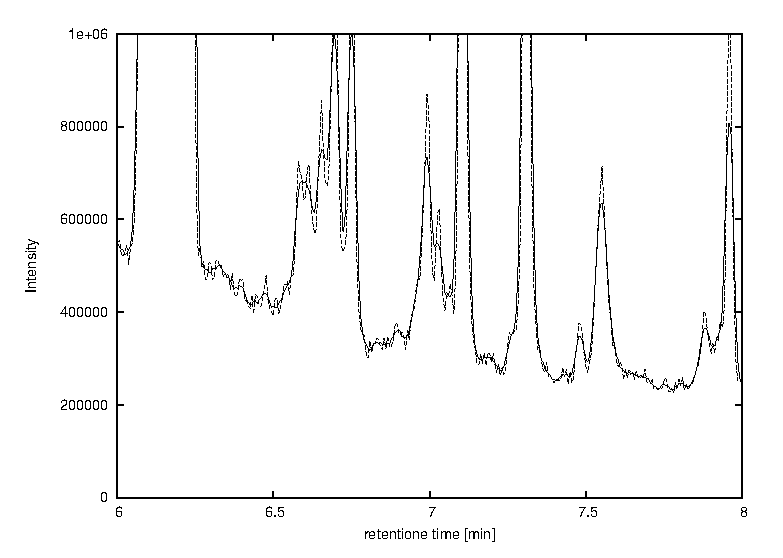
\includegraphics{graphics/pyms-test/tic_mean_smoothed.eps}
\caption{The effect of the 5-point mean moving window average smoothing
on the TIC from 'a0806\_140' data set. The segment 6.3-7.0 minutes is
shown. The original TIC is shown in full line, while the smoothed TIC
is shown in dashed line}
\label{fig:smoothed-mean}
\end{center}
\end{figure}

\begin{figure}[htp]
\begin{center}
\includegraphics{graphics/pyms-test/tic_median_smoothed.eps}
\caption{The effect of the 5-point median moving window average smoothing
on the TIC from 'a0806\_140' data set. The segment 6.3-7.0 minutes is
shown. The original TIC is shown in full line, while the smoothed TIC
is shown in dashed line}
\label{fig:smoothed-median}
\end{center}
\end{figure}

\section{Time strings}
\label{sec:time-string}

A time string is specification of time interval, that takes the format
'NUMBERs' or 'NUMBERm' for time interval in seconds or minutes. For
example, these are valid time strings: '10s' (10 seconds) and '0.2m'
(0.2 minutes).

\section{\label{sec:baseline_correction}Baseline correction}

\noindent
[ {\em This example is in pyms-test/21} ]

Baseline distortion originating from instrument imperfections and experimental
setup is often observed in mass spectrometry data, and off-line baseline correction
is an important part of data pre-processing. There are many approaches for
baseline correction. One advanced approach is based top-hat transform developed
in mathematical morphology \cite{serra83}, and used extensively in digital image
processing for tasks such as image enhancement.  Top-hat baseline correction was
previously applied in proteomics based mass spectrometry \cite{sauve04}.

PyMS currently implements only top-hat baseline corrector, using the SciPy
package 'ndimage'. For this feature to be available either SciPy (Scientific
Tools for Python \cite{scipy}) must be installed, or the local versions of
scipy's ndimage must be installed. For the SciPy/ndimage installation
instructions please see the section \ref{subsec:scipy-ndmage}.

Application of the top-hat baseline corrector requires the size of the structural
element to be specified. The structural element needs to be larger than the
features one wants to retain in the spectrum after the top-hat transform.
In the example below, the top-hat baseline corrector is applied to the TIC
of the data set 'a0806\_140.CDF', with the structural element of 1.5 minutes:

\begin{verbatim}
from pyms.IO.ANDI.Class import ChemStation
from pyms.Noise.Window import window_smooth
from pyms.Baseline.TopHat import tophat

andi_file = "/home/current/proj/PyMS/pyms-data/a0806_140.CDF"
andi_data = ChemStation(andi_file)

# get the TIC
tic = andi_data.get_tic()

# apply 5-point moving window smoothing & baseline corrector
tic = window_smooth(tic, window=5)
tic_bc = tophat(tic, struct="1.5m")

# save the original and baseline corrected TICs
tic.write("output/tic.dat",minutes=True)
tic_bc.write("output/tic_bc.dat",minutes=True)
\end{verbatim}

\noindent
The original and baseline corrected TICs are saved as files 'tic.dat' and
'tic\_bc.dat', in the directory 'output/'. Running this script produces the
following output:

\begin{verbatim}
$ python proc.py
 -> Processing netCDF file '/home/current/proj/PyMS/pyms-data/a0806_140.CDF'
    [ 3236 scans, masses from 50 to 550 ]
 -> Window smoothing (mean): the wing is 2 point(s)
 -> Top-hat: structural element is 262 point(s)
\end{verbatim}

\noindent
The plot of the original TIC and baseline corrected TIC is shown in
Figure \ref{fig:bc-tophat}.

\begin{figure}[htp]
\begin{center}
\includegraphics{graphics/pyms-test/tic_bc_tophat.eps}
\caption{The effect of the top-hat baseline corrector with the 1.5 minute
structural element on the TIC for the data 'a0806\_140.CDF'.  The original
TIC is shown in dashed line, while the baseline corrected TIC is shown in
full line.}
\label{fig:bc-tophat}
\end{center}
\end{figure}

It should be noted that top-hat baseline correction can be applied to any
ion chromatogram object (ie. m/z channel ion chromatogram), not only TIC.



\bibliography{bibtex/refbase}
\bibliographystyle{unsrt}

\backmatter
\printindex

\end{document}

